\documentclass[11pt]{article}
%

\usepackage{amsmath, amssymb, amsthm, enumerate}
\usepackage{graphicx, caption, subcaption}
\usepackage{xcolor}
\usepackage{cancel} %
\usepackage[pagebackref]{hyperref}

\usepackage{xspace}


\usepackage{tikz}
\usetikzlibrary{arrows.meta}

%
\definecolor{diagramred}{RGB}{178,32,45}
\definecolor{diagramgreen}{RGB}{0,108,72}
\definecolor{diagramblue}{RGB}{166,206,227}




%
%

%
\usepackage[margin=1.5in, marginparwidth=1.3in]{geometry}

%
\usepackage{titlesec}
\setcounter{secnumdepth}{3}

%


\theoremstyle{plain}
\newtheorem{thm}{Theorem}[section]
\newtheorem{prop}[thm]{Proposition}
\newtheorem{lemma}[thm]{Lemma}
\newtheorem{sublemma}[thm]{Sublemma}
\newtheorem{claim}[thm]{Claim}
\newtheorem{cor}[thm]{Corollary}
\newtheorem{fact}[thm]{Fact}
\newtheorem{conj}[thm]{Conjecture}


\theoremstyle{definition}
\newtheorem{defn}[thm]{Definition}
\newtheorem{assumption}[thm]{Assumption}
\newtheorem{operation}[thm]{Operation}
\newtheorem{construction}[thm]{Construction}
\newtheorem{question}[thm]{Question}
\newtheorem{problem}[thm]{Problem}


%
\newtheorem{rmkx}[thm]{Remark}
\newenvironment{rmk}
{\pushQED{\qed}\renewcommand{\qedsymbol}{$\triangle$}\rmkx}
{\popQED\endrmkx}

\newtheorem{examplex}[thm]{Example}
\newenvironment{example}
{\pushQED{\qed}\renewcommand{\qedsymbol}{$\triangle$}\examplex}
{\popQED\endexamplex}

%
%
%
\newenvironment{proofclaim}[1][Proof]{\begin{proof}[#1]\renewcommand*{\qedsymbol}{\(\square\)}}{\end{proof}}


%
\renewcommand\qedsymbol{$\blacksquare$} 

\newcommand{\barH}{\overline{\mathcal{H}}}
\newcommand{\barPH}{\overline{\mathbb{P}\mathcal{H}}}
\newcommand{\barMg}{\overline{\mathcal{M}}_g}
\newcommand{\barMgn}{\overline{\mathcal{M}}_{g,n}}
\newcommand{\barM}{\overline{\mathcal{M}}}
\newcommand{\C}{\mathbb{C}}
\newcommand{\Z}{\mathbb{Z}}
\newcommand{\R}{\mathbb{R}}
\newcommand{\Q}{\mathbb{Q}}
\newcommand{\E}{\mathbb{E}}
\newcommand\supp{\operatorname{supp}}

\newcommand{\M}{\mathcal{M}}
\newcommand{\calM}{\mathcal{M}}
\newcommand{\calN}{\mathcal{N}}
\newcommand{\K}{\mathcal{K}}
\newcommand{\T}{\mathcal{T}}
\newcommand{\calT}{\mathcal{T}}
\newcommand{\calQ}{\mathcal{Q}}

\newcommand\ninf{n \to \infty}

\renewcommand{\H}{\mathcal{H}}
\renewcommand{\P}{\mathbb{P}}
\renewcommand{\Re}{\operatorname{Re}}
\renewcommand{\Im}{\operatorname{Im}}
\newcommand{\lcm}{\operatorname{lcm}}
\newcommand{\tr}{\operatorname{Trace}}
\newcommand{\area}{\operatorname{area}}
\newcommand{\vol}{\operatorname{vol}}
%

\newcommand\RR{\mathbb{R}}
\newcommand\QQ{\mathbb{Q}}
\newcommand\CC{\mathbb{C}}

\newcommand{\Mgn}{\overline{\mathcal{M}}_{g,n}}
\newcommand\St[1][(\mu)]{\mathcal{H}#1}
%

\newcommand{\TM}{Teichm\"uller\xspace}
\newcommand{\osc}{\operatorname{osc}}



%



 
%
%
%
%
%

\title{Problem for First Proof, 3rd batch }  

%
\begin{document}
\begin{center}
{\large Benjamin Dozier, Sidhanth Raman, and Carlos Serv\'an}
\end{center}
\begin{proof}
  %

We will show the result for small $t$; by analyticity of the family, it then follows for all $t$.    For convenience, denote by $\M_c$ the factor $\M_{g_i,n_i}$.  Since $\partial V_0$ is positive dimensional, it must vary on some other factor $\M_{v}$.   Going forward, we will label boundary strata by the multi-curve (considered up to action of the mapping class group) pinched, rather than the dual graph.  Let $\Lambda$ be the multi-curve corresponding to the dual graph $\Gamma$, and then denote by $\Delta_\Lambda$ the boundary stratum $\Delta_\Gamma$.


      
    
    Fix a point $X \in \partial V_0$.  The image of the projection of $\pi_v:\partial V_0 \to \M_v$ is a totally geodesic subvariety (\cite[Theorem 1.4]{bdr24} or \cite[Theorem 1.3]{aw24}) of positive dimension, so it is non-compact (e.g. by using the $GL_2(\R)$ action).  Consider a degeneration in this factor (which may lead to degeneration in other factors, but not in $\M_c$, since it is $0$-dimensional there).  This lands at $X'$ in some more degenerate boundary stratum $\Delta_{\Lambda \cup \Lambda'}$, obtained from $\Delta_\Lambda$ by further pinching some multi-curve $\Lambda'$.  By  \cite[Theorem 1.6 (4)]{aw24}, $\Lambda$ is a union of disjoint equivalence classes (in their sense), since $X$ is in closure of $V_0$, and $\Lambda$ is the multi-curve pinched at $X$. And so is $\Lambda \cup \Lambda'$, since $X'$ is in closure of $V_0$.  It follows that $\Lambda'$ is also a union of disjoint equivalence classes.  Then by \cite[Corollary 3.17]{aw24}, nearby $X'$ we can unpinch the nodes corresponding to $\Lambda$.  This means that locally near $X'$, the boundary of $\bar V_0 \cap \Delta_{\Lambda'}$ in $\Delta_{\Lambda \cup \Lambda'}$ equals $\bar V_0 \cap \Delta_{\Lambda \cup \Lambda'}$.     
    
    Now we consider other elements $V_t$ of the family.  By (i), we get a family in $\Delta_\Lambda$ deforming the boundary of $V_0$ there.  Similarly, we get a family in $\Delta_{\Lambda \cup \Lambda'}$ and one in $\Delta_{\Lambda'}$, each deforming the boundaries of $V_0$ in those respective strata. 
    By (ii), the relevant nodes can be smoothed at other elements of the family, locally near $X'$, %
    %
   i.e.  for a small open neighborhood $U$ of $X'$,
    \begin{align}
        \overline{\bar V_t \cap \Delta_{\Lambda}} \cap \Delta_{\Lambda \cup \Lambda'} \cap U= \bar V_t \cap \Delta_{\Lambda \cup \Lambda'} \cap U. \label{eq:bdy-mon-lam}
    \end{align}
 and, similarly (now also using the result of the previous paragraph), we get
    \begin{align}
        \overline{\bar V_t \cap \Delta_{\Lambda'}} \cap \Delta_{\Lambda \cup \Lambda'} \cap U = \bar V_t \cap \Delta_{\Lambda \cup \Lambda'} \cap U. \label{eq:bdy-mon-lam'}
    \end{align}


       \begin{figure}
        \centering
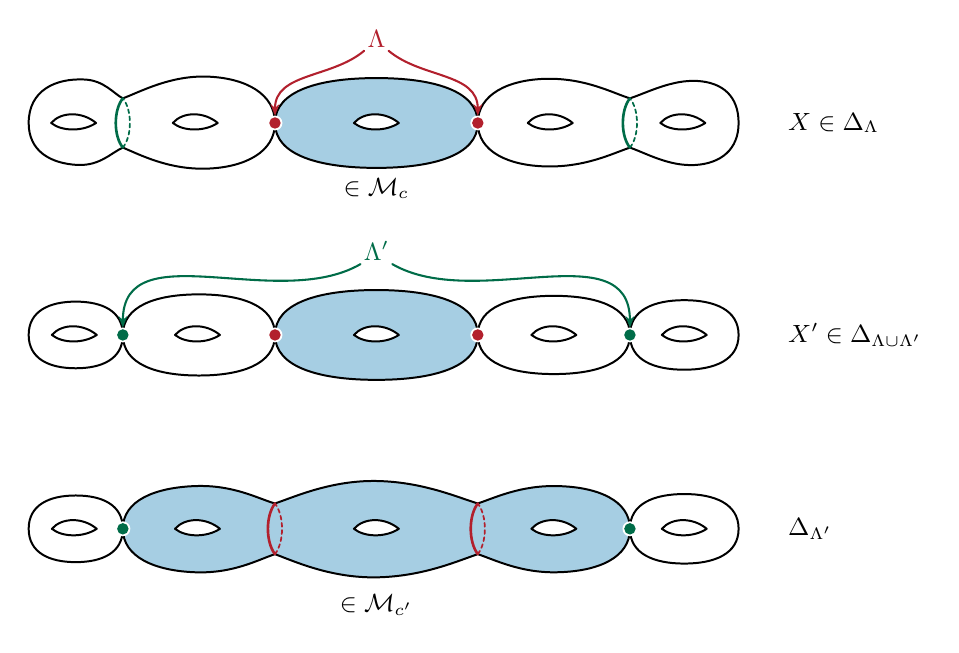
\begin{tikzpicture}[
    x=0.92cm,
    y=0.92cm,
    surface/.style={
        draw=black,
        fill=white,
        line width=0.72pt,
        line cap=round,
        line join=round
    },
    blue surface/.style={
        surface,
        fill=diagramblue
    },
    handle hole/.style={
        draw=black,
        fill=white,
        line width=0.72pt,
        line cap=round,
        line join=round
    },
    cut front/.style={
        line width=0.95pt,
        line cap=round
    },
    cut back/.style={
        line width=0.62pt,
        line cap=round,
        dash pattern=on 1.4pt off 1.2pt
    },
    set arrow/.style={
        -{Stealth[length=4.2pt,width=3.2pt]},
        line width=0.75pt,
        line cap=round
    },
    every node/.style={
        font=\small
    }
]

%
%
%

%
%
\newcommand{\ovalcomponent}[5][surface]{%
    \begingroup
    \pgfmathsetmacro{\L}{#2}
    \pgfmathsetmacro{\R}{#3}
    \pgfmathsetmacro{\Y}{#4}
    \pgfmathsetmacro{\H}{#5}
    \pgfmathsetmacro{\D}{\R-\L}
    \pgfmathsetmacro{\M}{(\L+\R)/2}
    \pgfmathsetmacro{\XL}{\L+0.22*\D}
    \pgfmathsetmacro{\XR}{\R-0.22*\D}
    \pgfmathsetmacro{\YT}{\Y+\H}
    \pgfmathsetmacro{\YB}{\Y-\H}
    \pgfmathsetmacro{\YU}{\Y+0.72*\H}
    \pgfmathsetmacro{\YD}{\Y-0.72*\H}

    \path[#1]
        (\L,\Y)
        .. controls (\L,\YU) and (\XL,\YT) ..
        (\M,\YT)
        .. controls (\XR,\YT) and (\R,\YU) ..
        (\R,\Y)
        .. controls (\R,\YD) and (\XR,\YB) ..
        (\M,\YB)
        .. controls (\XL,\YB) and (\L,\YD) ..
        (\L,\Y)
        -- cycle;
    \endgroup
}

%
\newcommand{\surfacehandle}[2]{%
    \begin{scope}[shift={(#1,#2)}]
        \path[handle hole]
            (-0.31,0.00)
            .. controls (-0.17,0.16) and (0.12,0.16) ..
            (0.31,0.00)
            .. controls (0.13,-0.12) and (-0.16,-0.12) ..
            (-0.31,0.00)
            -- cycle;
    \end{scope}%
}

%
%
%
\newcommand{\cutcurve}[4]{%
    \begingroup
    \pgfmathsetmacro{\YM}{(#2+#3)/2}
    \pgfmathsetmacro{\YML}{\YM-0.18}
    \pgfmathsetmacro{\YMU}{\YM+0.18}

    \path[cut front,draw=#4]
        (#1,#2)
        .. controls ({#1-0.13},\YML)
                    and ({#1-0.13},\YMU) ..
        (#1,#3);

    \path[cut back,draw=#4]
        (#1,#2)
        .. controls ({#1+0.13},\YML)
                    and ({#1+0.13},\YMU) ..
        (#1,#3);
    \endgroup
}

%
\newcommand{\colornode}[3]{%
    \fill[white] (#1,#2) circle[radius=2.7pt];
    \fill[draw=#3,fill=#3] (#1,#2) circle[radius=1.85pt];
}

%
%
%

\begin{scope}[yshift=3mm]

%
\path[surface]
    (0.25,5.60)
    .. controls (0.25,6.05) and (0.62,6.22) ..
    (1.02,6.20)
    .. controls (1.29,6.19) and (1.43,6.00) ..
    (1.55,5.94)
    .. controls (1.77,6.02) and (2.20,6.26) ..
    (2.72,6.24)
    .. controls (3.25,6.22) and (3.65,6.00) ..
    (3.65,5.60)
    .. controls (3.65,5.20) and (3.24,4.99) ..
    (2.72,4.97)
    .. controls (2.18,4.95) and (1.77,5.17) ..
    (1.55,5.26)
    .. controls (1.39,5.19) and (1.24,5.01) ..
    (0.93,5.02)
    .. controls (0.55,5.04) and (0.25,5.21) ..
    (0.25,5.60)
    -- cycle;

%
\ovalcomponent[blue surface]{3.65}{6.45}{5.60}{0.62}

%
\path[surface]
    (6.45,5.60)
    .. controls (6.45,6.00) and (6.88,6.20) ..
    (7.40,6.21)
    .. controls (7.94,6.22) and (8.32,6.01) ..
    (8.55,5.94)
    .. controls (8.79,6.02) and (9.13,6.20) ..
    (9.48,6.18)
    .. controls (9.83,6.16) and (10.05,5.97) ..
    (10.05,5.60)
    .. controls (10.05,5.23) and (9.80,5.04) ..
    (9.45,5.02)
    .. controls (9.09,5.00) and (8.78,5.18) ..
    (8.55,5.26)
    .. controls (8.31,5.18) and (7.94,4.99) ..
    (7.40,5.00)
    .. controls (6.88,5.01) and (6.45,5.20) ..
    (6.45,5.60)
    -- cycle;

%
\cutcurve{1.55}{5.26}{5.94}{diagramgreen}
\cutcurve{8.55}{5.26}{5.94}{diagramgreen}

%
\surfacehandle{0.87}{5.60}
\surfacehandle{2.55}{5.60}
\surfacehandle{5.05}{5.60}
\surfacehandle{7.45}{5.60}
\surfacehandle{9.28}{5.60}

%
\colornode{3.65}{5.60}{diagramred}
\colornode{6.45}{5.60}{diagramred}

%
\node[text=diagramred,inner sep=1pt] (Lambda)
    at (5.05,6.76) {$\Lambda$};

\draw[set arrow,draw=diagramred]
    (Lambda.south west)
    to[out=220,in=90] (3.65,5.70);

\draw[set arrow,draw=diagramred]
    (Lambda.south east)
    to[out=-40,in=90] (6.45,5.70);

%
\node at (5.05,4.70) {$\in\mathcal M_c$};

%
\node[anchor=west] at (10.60,5.60)
    {$X\in\Delta_{\Lambda}$};

\end{scope}

%
%
%

\ovalcomponent{0.25}{1.55}{3.00}{0.46}
\ovalcomponent{1.55}{3.65}{3.00}{0.56}

%
\ovalcomponent[blue surface]{3.65}{6.45}{3.00}{0.62}

\ovalcomponent{6.45}{8.55}{3.00}{0.54}
\ovalcomponent{8.55}{10.05}{3.00}{0.48}

%
\surfacehandle{0.88}{3.00}
\surfacehandle{2.58}{3.00}
\surfacehandle{5.05}{3.00}
\surfacehandle{7.50}{3.00}
\surfacehandle{9.30}{3.00}

%
\colornode{1.55}{3.00}{diagramgreen}
\colornode{8.55}{3.00}{diagramgreen}

%
\colornode{3.65}{3.00}{diagramred}
\colornode{6.45}{3.00}{diagramred}

%
\node[text=diagramgreen,inner sep=1pt] (Lambdap)
    at (5.05,4.16) {$\Lambda'$};

\draw[set arrow,draw=diagramgreen]
    (Lambdap.south west)
    to[out=210,in=90] (1.55,3.10);

\draw[set arrow,draw=diagramgreen]
    (Lambdap.south east)
    to[out=-30,in=90] (8.55,3.10);

%
\node[anchor=west] at (10.60,3.00)
    {$X'\in\Delta_{\Lambda\cup\Lambda'}$};

%
%
%

\begin{scope}[yshift=-3mm]

%
\ovalcomponent{0.25}{1.55}{0.65}{0.46}

%
%
\path[blue surface]
    (1.55,0.65)
    .. controls (1.55,1.04) and (1.99,1.22) ..
    (2.55,1.24)
    .. controls (3.08,1.26) and (3.43,1.06) ..
    (3.65,1.00)
    .. controls (3.92,1.09) and (4.42,1.32) ..
    (5.05,1.31)
    .. controls (5.69,1.30) and (6.18,1.08) ..
    (6.45,1.00)
    .. controls (6.69,1.08) and (7.04,1.25) ..
    (7.54,1.24)
    .. controls (8.11,1.23) and (8.55,1.04) ..
    (8.55,0.65)
    .. controls (8.55,0.25) and (8.11,0.06) ..
    (7.54,0.05)
    .. controls (7.04,0.04) and (6.69,0.22) ..
    (6.45,0.30)
    .. controls (6.18,0.21) and (5.69,-0.01) ..
    (5.05,-0.02)
    .. controls (4.42,-0.03) and (3.92,0.20) ..
    (3.65,0.30)
    .. controls (3.43,0.23) and (3.08,0.03) ..
    (2.55,0.05)
    .. controls (1.99,0.07) and (1.55,0.26) ..
    (1.55,0.65)
    -- cycle;

%
\ovalcomponent{8.55}{10.05}{0.65}{0.48}

%
\cutcurve{3.65}{0.30}{1.00}{diagramred}
\cutcurve{6.45}{0.30}{1.00}{diagramred}

%
\surfacehandle{0.88}{0.65}
\surfacehandle{2.58}{0.65}
\surfacehandle{5.05}{0.65}
\surfacehandle{7.50}{0.65}
\surfacehandle{9.30}{0.65}

%
\colornode{1.55}{0.65}{diagramgreen}
\colornode{8.55}{0.65}{diagramgreen}

%
\node at (5.05,-0.40) {$\in\mathcal M_{c'}$};

%
\node[anchor=west] at (10.60,0.65)
    {$\Delta_{\Lambda'}$};

\end{scope}

\end{tikzpicture}
        \caption{ Degenerations used in the proof. 
        }
        \label{fig:degen
        }
      \end{figure}

      
    
    %
    Note that $\M_c$ is also a factor in $\Delta_{\Lambda\cup \Lambda'}$, since the degeneration corresponding to $\Lambda'$ does not affect $\M_c$.  And the image of the projection $\pi_c: \bar V_0 \cap \Delta_{\Lambda \cup \Lambda'} \to \M_c$ is identical to image of the projection $\pi_c:\bar V_0 \cap \Delta_{\Lambda} \to \M_c$. 
    In $\Delta_{\Lambda'}$, $\M_c$ undegenerates into some factor $\M_{c'}$, i.e. $\M_c$ a factor in $\partial \M_{c'}$.   Now the image of the projection $\pi_{c'}: \bar V_0 \cap \Delta_{\Lambda'} \to \M_{c'}$ has dimension one (the dimension is $\ge 1$ since it admits a degeneration, to $\M_c$, by pinching $\Lambda$; the dimension is $\le 1$ is since it lies on the boundary of the surface $V_0$).   
    %
    Again by \cite[Theorem 1.7]{bdr24} or \cite[Theorem 1.3]{aw24}, the projection of $\bar V_0 \cap \Delta_{\Lambda'}$ to $\M_{c'}$ is totally geodesic. 
    By \cite{mcmullen09}, %
    this is holomorphically rigid.  In particular, $\pi_{c'}(\bar V_t \cap \Delta_{\Lambda'})$ does not depend on $t$, for $t$ in some small disc.
    But $\pi_c(\bar V_t \cap \Delta_{\Lambda \cup \Lambda'})$ is (locally, near $X'$) the boundary of this, since by \eqref{eq:bdy-mon-lam'}, this is true of the whole product.
    %
    %
    %
    %
    %
    %
    We conclude that $\pi_c(\bar V_t \cap \Delta_{\Lambda \cup \Lambda'})$  also does not depend on $t$.  


    
    Now we are assuming for each $t$ that $\pi_c(\bar V_t \cap \Delta_{\Lambda})$ consists of a single point, call it $Y_t$. Since $\Lambda'$ does not contain any curves on the $\M_c$ factor, and using \eqref{eq:bdy-mon-lam}, we get that $\pi_c(\bar V_t \cap \Delta_{\Lambda \cup \Lambda'})$ also must equal $\{Y_t\}$.
    %
    And since we saw in the previous paragraph that $\pi_c(\bar V_t \cap \Delta_{\Lambda \cup \Lambda'})$ does not depend on $t$, neither does $Y_t$.  

    



    
    %
    
    %
    %
    %
    %
    %
    %
    %
    
    %

    %
\end{proof}






{\footnotesize
\bibliographystyle{amsalpha}
  %
\providecommand{\bysame}{\leavevmode\hbox to3em{\hrulefill}\thinspace}
\providecommand{\MR}{\relax\ifhmode\unskip\space\fi MR }
%
\providecommand{\MRhref}[2]{%
  \href{http://www.ams.org/mathscinet-getitem?mr=#1}{#2}
}
\providecommand{\href}[2]{#2}
\begin{thebibliography}{McM09}

\bibitem[AW24]{aw24}
Francisco {Arana-Herrera} and Alex {Wright}, \emph{{The geometry of totally
  geodesic subvarieties of moduli spaces of Riemann surfaces}}, arXiv e-prints
  (2024), arXiv:2412.16330.

\bibitem[BDR24]{bdr24}
Frederik {Benirschke}, Benjamin {Dozier}, and John {Rached}, \emph{{The
  boundary of a totally geodesic subvariety of moduli space}}, arXiv e-prints.
  To appear in Journal of the European Math. Society. (2024), arXiv:2412.06765.

\bibitem[McM09]{mcmullen09}
Curtis~T. McMullen, \emph{Rigidity of {T}eichm\"uller curves}, Math. Res. Lett.
  \textbf{16} (2009), no.~4, 647--649. \MR{2525030}

\end{thebibliography}
 %
%
}
\end{document}
